\part{Logiciel d'annotation d'images}
\section{Objectif du logiciel}

Le but de la première partie est de réaliser un logiciel d’annotation d’images en python pour fournir un jeu de données à nôtre IA dans la seconde partie du projet.\\

Nous avons dû donner la possibilité à l'utilisateur d'encadrer une ou plusieurs parties de l'image puis de leur assigner une catégorie. Chaque cadre doit pouvoir être éditable, pour changer la catégorie ou supprimer le cadre. L’utilisateur doit pouvoir sauvegarder toutes ses annotations. En ce qui concerne les catégories il est nécessaire de pouvoir en importer, en ajouter ou en supprimer.

\section{Base de donnée}
Pour récolter les données nécessaires à l'entrainement de l'IA nous nous sommes rendu sur \href{https://www.kaggle.com/swann00/masque-vs-sans-masque}{kaggle.com} où nous avons recherché un jeu de données composé de différentes personnes. Nos critères étaient d'y trouver des personnes dans diverses situations, de différents âges, ethnies et en nombre varié pour avoir une diversité suffisante, afin d'éviter les problèmes liés à un jeu de données trop réduit. Cependant les images nous semblent petites, nous verrons dans la seconde partie du projet si elles conviennent bien à nos besoins.\\

Pour la partie annotation, nous avons enregistré pour chaque image dans un JSON, un identifiant unique, les coordonnées des zones annotées associées au titre d'une catégorie, sa taille ainsi que le chemin vers cette dernière. En revanche la sauvegarde n'est pas automatique, il faut enregistrer à la fin de chaque session d'annotation dans un fichier JSON.

\newpage
\section{Choix de conception}

\begin{description}
\item Méthodologie:
Pour mieux s'organiser au cours du projet nous avons utilisé l'outil de versioning git.
Cet outil nous a permis de travailler à plusieurs sur différentes branches en simultané et enfin de fusionner le tout pour avoir un produit tout le temps fonctionnel.

\item Technologies : \textbf{Python3.9.9}\\
Pour réaliser l'interface graphique de ce projet nous nous sommes plutôt rapprochés d'une librairie externe nommée Qt, développée en \textit{C++} qui selon nous est plus ergonomique que le GUI classique de Python \guillemotleft \textbf{tkinter}\guillemotright.\\
Qt est une librairie très puissante et moderne c'est pourquoi nous voulions en apprendre plus dessus.\\
Les différentes librairies utilisées au cours du projet sont :
    \begin{itemize}
        \item PySide6==6.2.1 (librairie Qt adapté pour python)
        \item Pillow==8.4.0 (redimensionner des images)
        \item Shapely==1.8.0 (intersections entre les rectangles)
    \end{itemize}
\end{description}



\section{Répartition des tâches}
Pour la répartition des tâches nous nous sommes organisés via GitHub et son système d'issues, mais aussi via Discord où nous recensions les bugs à réparer ainsi que les fonctionnalités à implémenter, nous passions par des phases de test où nous essayions de mettre le logiciel à l'épreuve pour détecter les bugs potentiels. \\

Antoine s'est occupé de l'import et de l'export des données et des catégories, Dylann de toute la gestion des zones d'annotations, leur chevauchement, leur affichage et Margaux de la gestion des catégories, l'ajout, la suppression et la modification.

\section{Comment utiliser}
NOTE: Pensez à mettre les droits d'exécution sur le fichier \textbf{build.sh} pour installer les dépendances et lancer l'application.

Pour lancer :
\begin{verbatim}
#!/bin/bash
chmod u+x build.sh
./build.sh
\end{verbatim}
\clearpage

\begin{itemize}
    \item Pour \textbf{ouvrir un fichier ou un dossier} via la menu-bar ou en effectuant un drag and drop sur la zone prévue à cet effet.
    \item Pour \textbf{ouvrir une image}, une fois le dossier ouvert, double-cliquez dessus et commencez à annoter.
    \item Pour \textbf{sélectionner une zone} vous pouvez appuyer sur clic gauche et étirer jusqu'à la taille souhaitée, la fenêtre de choix de categorie s'ouvre. Vous pouvez \textbf{séléctioner une categorie} et cliquer sur "Select category".
    \item Vous pouvez sélectionner plusieurs zones sur une même image.
    \item Pour \textbf{supprimer une annotation} faites clic droit sur la zone annotée de l'image.
    \item Pour \textbf{éditer une annotation} double-cliquez dessus, la fenêtre des choix de catégorie va apparaitre et vous pourrez éditer votre annotation.
    \item Pour \textbf{éditer une catégorie} double-cliquez dessus pour qu'elle devienne éditable, une fois la modification faite, appuyez sur "Change Category" pour valider le changement, qui se reportera dans le fichier JSON d'annotation.
    \item Pour \textbf{supprimer une categorie} selectionner là et cliquer sur "Delete category".
    \item Pour \textbf{ajouter  une categorie} écriver son nom dans la zone éditable en haut et cliquer sur "Ok".
    \item CTRL + S : Sauvegarder.
    \item CTRL + O : Ouvrir un fichier.
    \item CTRL + SHIFT + O : Ouvrir un dossier.
    \item CTRL + W : Quitter une image.
    \item CTRL + H : Ouvrir ce README.
\end{itemize}

\begin{center}
    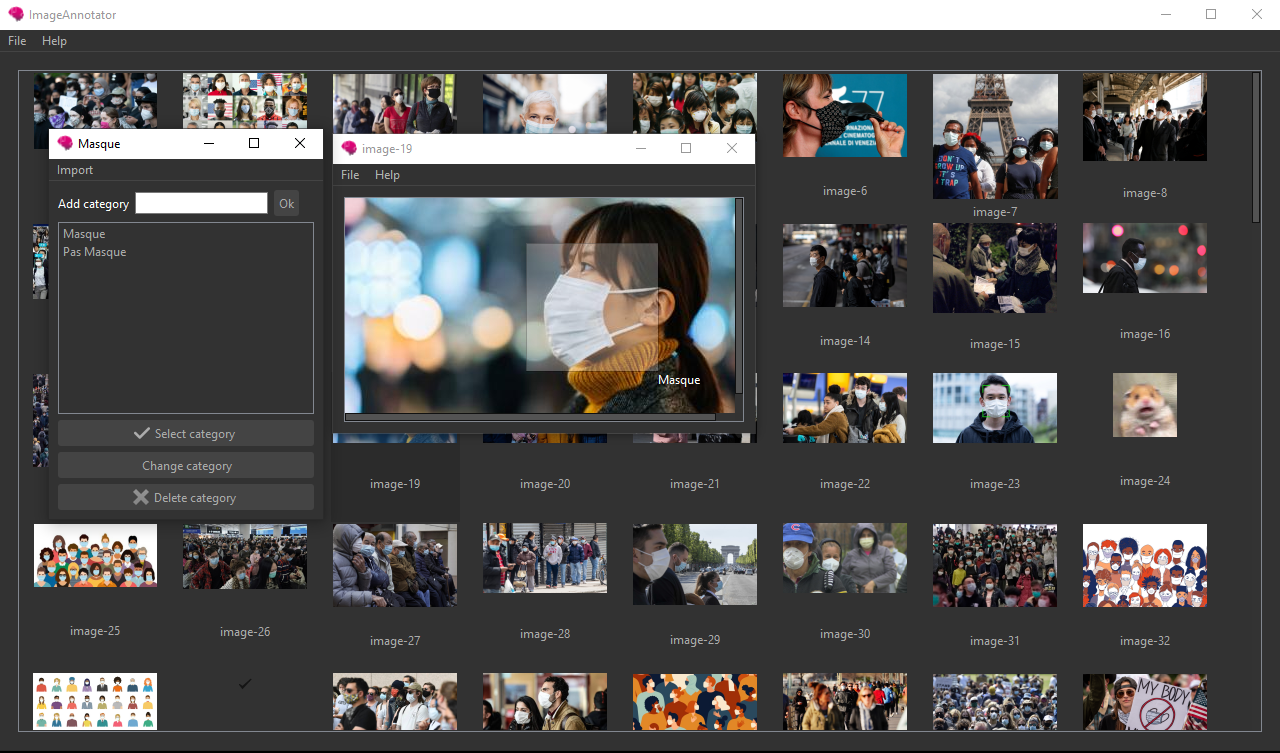
\includegraphics[scale=0.3]{resources/annotation.png}
    \captionof{figure}{Logiciel en action}
\end{center}


\section{Amélioration possible du logiciel}

Nous avons pensé à implémenter un système de Ctrl-Z Ctrl-Y à l'avenir sur l'édition des zones d'annotations, c'est une fonctionnalité qui paraît simple en apparence mais nous demande beaucoup de travail en arrière-plan, invisible pour l'utilisateur.
Nous avons testé le logiciel à la recherche de bug, ce qui a permis d'en régler plusieurs lors de cette période. Nous n'en avons plus trouvé après les corrections de ceux recensés. \\
Le projet étant très intéressant nous avons imaginé continuer le logiciel et peut-être faire en sorte d'annoter des vidéos pour que l'on puisse à partir d'une séquence obtenir une multitude d'images et entrainer l'IA sur celle-ci voir même sur des films.


\section{Conclusion du logiciel d'annotation}

Lors de cette première partie nous avons donc réalisé ce logiciel de façon à ce qu’il nous convienne pour travailler pour la seconde partie. Nous avons implémenté les fonctionnalités qui nous semblaient utiles, pour pouvoir annoter efficacement les images. En effet si nous avons un logiciel ergonomique, nous faciliterons la phase de création du jeu de données d'images, pour nourrir notre algorithme. \\

Cette partie nous a permis de prendre en main les librairies graphiques en python et de faire attention à l'efficacité du logiciel.
\newpage